\documentclass{article}
\usepackage{amsmath}
\usepackage{amssymb}
\usepackage[pdftex]{graphicx}
\usepackage[framed,numbered,autolinebreaks,useliterate]{mcode}
\lstset{breakatwhitespace=false}
\usepackage{pgfplots}

\pdfpagewidth 8.5in
\pdfpageheight 11in
\topmargin -1in
\headheight 0in
\headsep 0in
\textheight 8.5in
\textwidth 6.5in
\oddsidemargin 0in
\evensidemargin 0in 
\headheight 50pt
\headsep 0in
\footskip .75in

\title{STA 601 - Lab 6}
\author{Kedar Prabhudesai}
\date{October 25, 2013}

\begin{document}
\maketitle

\noindent {\underline{\textbf{Normalizing Constant:}}}\\

Given distribution,
\begin{eqnarray*}
\pi(\theta) \propto exp\left[-\frac{\theta^2}{2}\right] + \frac{1}{2}exp\left[-\frac{(\theta-3)^2}{2}\right]
\end{eqnarray*}

To find the Normalizing constant ($\kappa$), we can integrate the above equation.
\begin{eqnarray*}
\kappa &=& \int_0^\infty{exp\left[-\frac{\theta^2}{2}\right] + exp\left[-\frac{(\theta-3)^2}{2}\right]}d\theta\\
&=& \int_0^\infty{exp\left[-\frac{\theta^2}{2}\right]}d\theta + \frac{1}{2}\int_0^\infty{exp\left[-\frac{(\theta-3)^2}{2}\right]}d\theta\\
&=& \sqrt{2\pi}\int_0^\infty{\frac{1}{\sqrt{2\pi}}exp\left[-\frac{\theta^2}{2}\right]}d\theta + \frac{1}{2}\sqrt{2\pi}\int_0^\infty{\frac{1}{\sqrt{2\pi}}exp\left[-\frac{(\theta-3)^2}{2}\right]}d\theta\\
&=& \sqrt{2\pi} + \frac{1}{2}\sqrt{2\pi}\\
&=& \sqrt{2\pi}\left(1+\frac{1}{2}\right)\\
\therefore \kappa &=& \frac{3\sqrt{2\pi}}{2}
\end{eqnarray*}

\pagebreak

\noindent {\underline{\textbf{Metropolis-Hastings Algorithm:}}}\\

Start with $\theta^{(0)} = 0$
\begin{itemize}
\item Sample, $\theta' \sim \mathcal{N}(\theta^{(s)},\sigma_{cand})$
\item Compute acceptance ration, $r = \pi(\theta')/\pi(\theta^{(s)})$
\item Draw, $u \sim$ Uniform[$0,1$]. If $u < r$ $\theta^{(s+1)} = \theta'$, else $\theta^{(s+1)} = \theta^{(s)}$.\\
\end{itemize}

I used $\sigma_{cand} = 4,$ and I got an acceptance ratio of $43.54\%.$ Given below is the Histogram and a plot of the function. Since, my starting value was $0,$ which is in the sample range, I did not need Burn-In.

\begin{center}
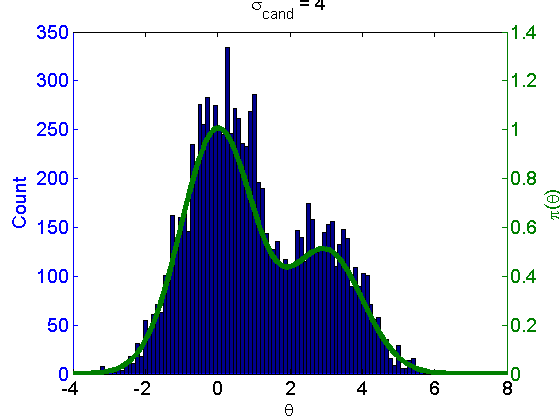
\includegraphics[scale=0.75]{AnalyticAndSampled4.png}\\
\end{center}

\pagebreak

Using $\sigma_{cand} = 0.05,$ we need lot more samples to cover the entire distribution, since we take very small steps. Hence we end up not sampling from the entire distribution.\\
\begin{center}
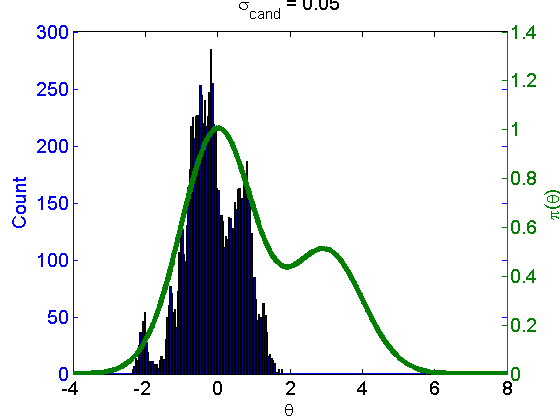
\includegraphics[scale=0.75]{AnalyticAndSampled005.png}\\
\end{center}

\pagebreak

Using $\sigma_{cand} = 8,$ makes our candidate distribution very wide and end up rejecting a lot of samples. Note that here we do cover our target distribution but it is very inefficient. For this chain my acceptance probability was $20.49\%$\\
\begin{center}
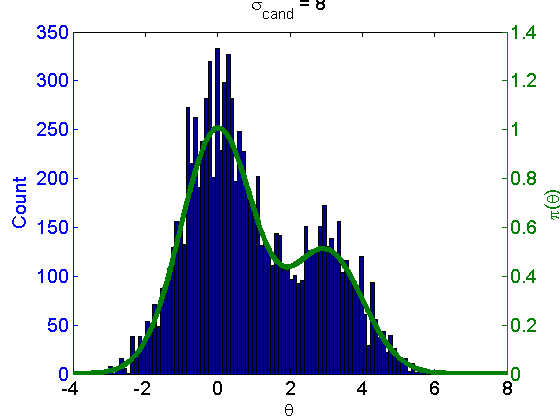
\includegraphics[scale=0.75]{AnalyticAndSampled8.png}\\
\end{center}

\pagebreak

Using $\sigma_{cand} = 100,$ makes our candidate distribution even wider and it is the worst case scenario. Now, we are drawing from a candidate distribution which has a huge variance, hence we are going to reject most of the samples. For the following plot, I got an acceptance probability of $1.83\%$\\
\begin{center}
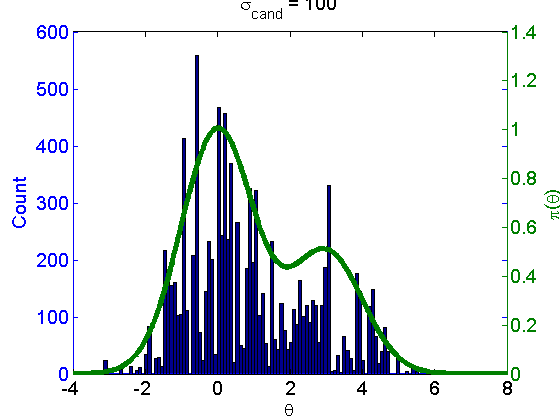
\includegraphics[scale=0.75]{AnalyticAndSampled100.png}\\
\end{center}


\pagebreak
\noindent {\Large\underline{\textbf{Appendix:}}}\\
\lstinputlisting{C:/Users/ksp6/Documents/Classes/2013-Fall/STA601-BayesAndModStats/labs/lab6/sta601_ksp6_Lab6.m}

\end{document}